\tikzset{every picture/.style={line width=0.75pt}} %set default line width to 0.75pt        

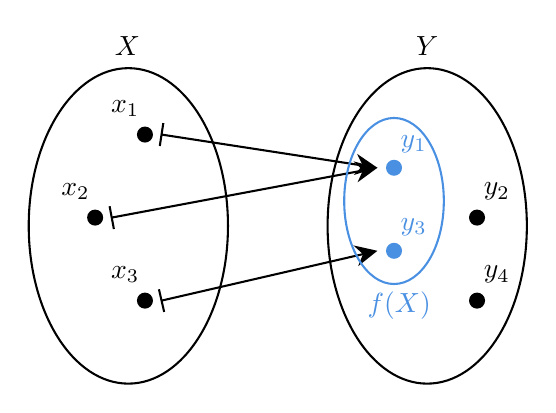
\begin{tikzpicture}[x=0.75pt,y=0.75pt,yscale=-1,xscale=1]
%uncomment if require: \path (0,308); %set diagram left start at 0, and has height of 308

%Shape: Ellipse [id:dp8584080168945698] 
\draw   (160,124) .. controls (160,82.03) and (181.49,48) .. (208,48) .. controls (234.51,48) and (256,82.03) .. (256,124) .. controls (256,165.97) and (234.51,200) .. (208,200) .. controls (181.49,200) and (160,165.97) .. (160,124) -- cycle ;
%Straight Lines [id:da9209150729175881] 
\draw    (216,80) ;

\draw [shift={(216,80)}, rotate = 0] [color={rgb, 255:red, 0; green, 0; blue, 0 }  ][fill={rgb, 255:red, 0; green, 0; blue, 0 }  ][line width=0.75]      (0, 0) circle [x radius= 3.35, y radius= 3.35]   ;
%Straight Lines [id:da7784202535308219] 
\draw [color={rgb, 255:red, 74; green, 144; blue, 226 }  ,draw opacity=1 ]   (336,96) ;

\draw [shift={(336,96)}, rotate = 0] [color={rgb, 255:red, 74; green, 144; blue, 226 }  ,draw opacity=1 ][fill={rgb, 255:red, 74; green, 144; blue, 226 }  ,fill opacity=1 ][line width=0.75]      (0, 0) circle [x radius= 3.35, y radius= 3.35]   ;
%Shape: Ellipse [id:dp3856498056795209] 
\draw   (304,124) .. controls (304,82.03) and (325.49,48) .. (352,48) .. controls (378.51,48) and (400,82.03) .. (400,124) .. controls (400,165.97) and (378.51,200) .. (352,200) .. controls (325.49,200) and (304,165.97) .. (304,124) -- cycle ;
%Straight Lines [id:da4011502733578831] 
\draw    (200,120) -- (326.03,96.37) ;
\draw [shift={(328,96)}, rotate = 529.38] [fill={rgb, 255:red, 0; green, 0; blue, 0 }  ][line width=0.75]  [draw opacity=0] (10.72,-5.15) -- (0,0) -- (10.72,5.15) -- (7.12,0) -- cycle    ;
\draw [shift={(200,120)}, rotate = 529.38] [color={rgb, 255:red, 0; green, 0; blue, 0 }  ][line width=0.75]    (0,5.59) -- (0,-5.59)   ;
%Straight Lines [id:da7099724823991076] 
\draw [color={rgb, 255:red, 74; green, 144; blue, 226 }  ,draw opacity=1 ]   (336,136) ;

\draw [shift={(336,136)}, rotate = 0] [color={rgb, 255:red, 74; green, 144; blue, 226 }  ,draw opacity=1 ][fill={rgb, 255:red, 74; green, 144; blue, 226 }  ,fill opacity=1 ][line width=0.75]      (0, 0) circle [x radius= 3.35, y radius= 3.35]   ;
%Straight Lines [id:da4810899906621904] 
\draw    (192,120) ;

\draw [shift={(192,120)}, rotate = 0] [color={rgb, 255:red, 0; green, 0; blue, 0 }  ][fill={rgb, 255:red, 0; green, 0; blue, 0 }  ][line width=0.75]      (0, 0) circle [x radius= 3.35, y radius= 3.35]   ;
%Straight Lines [id:da1387493271002489] 
\draw    (216,160) ;

\draw [shift={(216,160)}, rotate = 0] [color={rgb, 255:red, 0; green, 0; blue, 0 }  ][fill={rgb, 255:red, 0; green, 0; blue, 0 }  ][line width=0.75]      (0, 0) circle [x radius= 3.35, y radius= 3.35]   ;
%Straight Lines [id:da07664909250691976] 
\draw    (376,120) ;

\draw [shift={(376,120)}, rotate = 0] [color={rgb, 255:red, 0; green, 0; blue, 0 }  ][fill={rgb, 255:red, 0; green, 0; blue, 0 }  ][line width=0.75]      (0, 0) circle [x radius= 3.35, y radius= 3.35]   ;
%Straight Lines [id:da9651324228114074] 
\draw    (376,160) ;

\draw [shift={(376,160)}, rotate = 0] [color={rgb, 255:red, 0; green, 0; blue, 0 }  ][fill={rgb, 255:red, 0; green, 0; blue, 0 }  ][line width=0.75]      (0, 0) circle [x radius= 3.35, y radius= 3.35]   ;
%Straight Lines [id:da7557341854466749] 
\draw    (224,160) -- (326.05,136.45) ;
\draw [shift={(328,136)}, rotate = 527.01] [fill={rgb, 255:red, 0; green, 0; blue, 0 }  ][line width=0.75]  [draw opacity=0] (10.72,-5.15) -- (0,0) -- (10.72,5.15) -- (7.12,0) -- cycle    ;
\draw [shift={(224,160)}, rotate = 527.01] [color={rgb, 255:red, 0; green, 0; blue, 0 }  ][line width=0.75]    (0,5.59) -- (0,-5.59)   ;
%Straight Lines [id:da17659401986386492] 
\draw    (224,80) -- (326.02,95.7) ;
\draw [shift={(328,96)}, rotate = 188.75] [fill={rgb, 255:red, 0; green, 0; blue, 0 }  ][line width=0.75]  [draw opacity=0] (10.72,-5.15) -- (0,0) -- (10.72,5.15) -- (7.12,0) -- cycle    ;
\draw [shift={(224,80)}, rotate = 188.75] [color={rgb, 255:red, 0; green, 0; blue, 0 }  ][line width=0.75]    (0,5.59) -- (0,-5.59)   ;
%Shape: Ellipse [id:dp8087351065679074] 
\draw  [color={rgb, 255:red, 74; green, 144; blue, 226 }  ,draw opacity=1 ] (312,112) .. controls (312,89.91) and (322.75,72) .. (336,72) .. controls (349.25,72) and (360,89.91) .. (360,112) .. controls (360,134.09) and (349.25,152) .. (336,152) .. controls (322.75,152) and (312,134.09) .. (312,112) -- cycle ;

% Text Node
\draw (207.5,37.5) node   {$X$};
% Text Node
\draw (352,37.5) node   {$Y$};
% Text Node
\draw (338.5,162.5) node [color={rgb, 255:red, 74; green, 144; blue, 226 }  ,opacity=1 ]  {$f( X)$};
% Text Node
\draw (206.5,67.5) node   {$x_{1}$};
% Text Node
\draw (182.5,107.5) node   {$x_{2}$};
% Text Node
\draw (206.5,147.5) node   {$x_{3}$};
% Text Node
\draw (345.5,84.5) node [color={rgb, 255:red, 74; green, 144; blue, 226 }  ,opacity=1 ]  {$y_{1}$};
% Text Node
\draw (345.5,124.5) node [color={rgb, 255:red, 74; green, 144; blue, 226 }  ,opacity=1 ]  {$y_{3}$};
% Text Node
\draw (385.5,107.5) node [color={rgb, 255:red, 0; green, 0; blue, 0 }  ,opacity=1 ]  {$y_{2}$};
% Text Node
\draw (385.5,147.5) node [color={rgb, 255:red, 0; green, 0; blue, 0 }  ,opacity=1 ]  {$y_{4}$};

\end{tikzpicture}